% IEEE Transactions on Pattern Analysis and Machine Intelligence (TPAMI)
% manuscript template. Replace all bracketed placeholder text before submission.
\documentclass[10pt,journal,compsoc]{IEEEtran}

% Core mathematics and typography
\usepackage{amsmath,amssymb,amsfonts}
\usepackage{amsthm}
\usepackage{mathtools}
\usepackage{graphicx}
% Font expansion and protrusion keep justified lines from opening wide gaps.
\usepackage{microtype}
\usepackage{booktabs}
\usepackage{multirow}
\usepackage{array}
\usepackage{placeins}
% Labels of the supplementary material, for references such as Table S1.
\usepackage{xr}
\externaldocument[S-]{supplementary}
\usepackage{tikz}
\usetikzlibrary{shapes.geometric,shapes.arrows,arrows.meta,positioning}
% IEEEtran's compsoc headings, with the same natural spacing but less stretch,
% so that a short column spreads its spare space over paragraph breaks and
% displays instead of opening wide gaps above headings.
\makeatletter
\def\section{\@startsection{section}{1}{\z@}{-3.5ex plus -0.5ex minus -1.5ex}%
{0.7ex plus 0.2ex minus 0ex}{\normalfont\sublargesize\sffamily\bfseries\scshape}}
\def\subsection{\@startsection{subsection}{2}{\z@}{-3.5ex plus -0.5ex minus -1.5ex}%
{0.7ex plus 0.1ex minus 0ex}{\normalfont\normalsize\sffamily\bfseries}}
\makeatother
\usepackage{cite}
\usepackage{xcolor}
\usepackage{url}

% Uncomment when algorithms are needed.
% \usepackage{algorithm}
% \usepackage{algorithmic}

% Uncomment for hyperlinks in the review/preprint version.
% \usepackage[hidelinks]{hyperref}

% Common theorem environments
\newtheorem{theorem}{Theorem}
\newtheorem{lemma}[theorem]{Lemma}
\newtheorem{proposition}[theorem]{Proposition}
\theoremstyle{definition}
\newtheorem{definition}{Definition}

% Convenient notation
\newcommand{\R}{\mathbb{R}}
\newcommand{\vect}[1]{\mathbf{#1}}
\DeclareMathOperator*{\argmax}{arg\,max}
\newcolumntype{L}[1]{>{\raggedright\arraybackslash}p{#1}}

\begin{document}

\title{Repairing the Teacher for Knowledge Distillation via Causally Screened Channel Edits}

% Anonymized for double-blind review; restore the author names and
% affiliations for the final version.
\author{Anonymous Authors%
\IEEEcompsocitemizethanks{
\IEEEcompsocthanksitem Manuscript received [Month Day, Year]; revised [Month Day, Year].}}

\markboth{IEEE Transactions on Pattern Analysis and Machine Intelligence,~Vol.~XX, No.~XX, September~2026}%
{Anonymous Authors: Repairing the Teacher for Knowledge Distillation}

\IEEEtitleabstractindextext{%
\begin{abstract}
Knowledge distillation (KD) passes a teacher's errors to its student,
and refining the loss cannot supply what the teacher never
learned. The main contribution of this paper is teacher repair, which
corrects the knowledge source itself before distillation and leaves the
KD objective unchanged. For designated target classes, the repair scores
convolutional channels by contrasting hard and correctly classified
images of the same class, keeps channels that are stable under
resampling and whose removal raises the target-class margin, and
fine-tunes only their parameters under output and feature preservation.
An edit is accepted only if validation target recall improves within a
small accuracy tolerance. It was evaluated with a compact CNN
teacher, ResNet-18 and ResNet-34 and a small CNN student in 52 settings
from 13 image-classification datasets, against classical KD, LoCa, DKD
and RLD. Selected repairs edited at most 4.2\% of the searched
channels. Where a repair was selected, the CNN teacher gained 0.87
percentage points (pp) in accuracy and 2.68 pp in target-class recall,
and 58\% of that recall gain reached the student. Over all 52 settings,
its student gained 0.23 pp in accuracy and 0.69 pp in target recall
(Wilcoxon signed-rank test, $p<0.01$) and reached 74.91\% accuracy and
61.78\% target recall, significantly above all four losses. The ResNet
teachers gained less target recall, 1.37 and 0.73 pp, yet 42\% and 56\% of
it still reached the student. A correction made in a few teacher
channels therefore carries through unchanged distillation, and repairing
the teacher complements refining the loss.
\end{abstract}

\begin{IEEEkeywords}
Causal intervention, class imbalance, convolutional neural networks,
image classification, knowledge distillation, model editing, model repair.
\end{IEEEkeywords}}

\maketitle

\section{Introduction}
\label{sec:introduction}

Knowledge distillation trains a compact student, $S$, to reproduce the
predictive distribution of a larger teacher, $T$~\cite{gou2021knowledge}. The
teacher's softened outputs capture class similarities and uncertainty that hard
labels omit. A small student can use this information to learn more effectively
than from data alone. For an input $x$ and $M\in\{S,T\}$, define the
temperature-scaled output distribution as
\begin{equation}
\label{eq:softmax-temperature}
p_M^{(\tau)}(x) \triangleq
\operatorname{softmax}\!\left(\frac{z_M(x)}{\tau}\right),
\end{equation}
where $z_M(x)$ denotes the logits produced by model $M$ and $\tau>0$ is the
temperature. Let $\mathcal{D}$ denote the underlying distribution of
input--label pairs $(x,y)$, where $y$ lies in the label set
$\mathcal{Y}=\{0,\ldots,C-1\}$ of $C$ classes. The standard
population knowledge-distillation objective is
\begin{equation}
\label{eq:kd}
\begin{aligned}
\mathcal{L}_{\mathrm{KD}}
&= \mathbb{E}_{(x,y)\sim\mathcal{D}}\!\left[
\alpha\,\mathcal{L}_{\mathrm{CE}}\!\left(y, p_S^{(1)}(x)\right)\right. \\
&\qquad\left. {}+ (1-\alpha)\tau^2 D_{\mathrm{KL}}\!\left(
p_T^{(\tau)}(x)\,\middle\|\,p_S^{(\tau)}(x)
\right)\right].
\end{aligned}
\end{equation}
In Eq.~\eqref{eq:kd}, the first term is the cross-entropy
$\mathcal{L}_{\mathrm{CE}}(y,p)=-\log p_y$ between the student's standard
output, $p_S^{(1)}(x)$, and the true label $y$. The second term aligns the student and teacher softened
outputs, $p_S^{(\tau)}(x)$ and $p_T^{(\tau)}(x)$, using Kullback--Leibler (KL)
divergence. The factor $\tau^2$ preserves the scale of the distillation
gradients, and $\alpha\in[0,1]$ balances the two
losses~\cite{hinton2015distilling}.

While Eq.~\eqref{eq:kd} is intuitive, achieving the ideal learning outcome remains challenging. We define the \emph{generalization error} and the
temperature-dependent \emph{fidelity gap} as follows:
\begin{equation}
\label{eq:generalization-error}
\mathcal{E}(f) \triangleq \mathbb{E}_{(x,y)\sim\mathcal{D}}
\mathbf{1}\!\left[\argmax_k f_k(x) \neq y\right],
\end{equation}
and
\begin{equation}
\label{eq:fidelity-gap}
\Phi_{\tau}(S,T) \triangleq \mathbb{E}_{x\sim\mathcal{D}}\,
D_{\mathrm{KL}}\!\left(
p_T^{(\tau)}(x)\,\middle\|\,p_S^{(\tau)}(x)
\right).
\end{equation}
The second term in Eq.~\eqref{eq:kd} is therefore
$(1-\alpha)\tau^2\Phi_{\tau}(S,T)$, so that $\Phi_{\tau}(S,T)=0$ exactly when
the student reproduces the teacher's temperature-$\tau$ predictive
distribution almost everywhere under $\mathcal{D}$. Three findings complicate
this as a goal: it is not attained in practice, the target itself is
unreliable on a subset of classes, and the deviation from it is structured
rather than random.

\vspace{-5pt}
\subsection{Fidelity is not attained, and is not the right target}
\label{sec:f1}

Suppose the student is expressive enough to realize the teacher, so that
$\inf_{\theta \in \Theta_S} \Phi_{\tau}(S_{\theta},T) = 0$ over its
parameter set $\Theta_S$. The solution
$\hat{\theta}$ found by SGD can nonetheless satisfy
$\Phi_{\tau}(S_{\hat{\theta}},T) \gg 0$: the obstruction is optimization, not
capacity. Fidelity and generalization are moreover not aligned, in the sense
that $\mathcal{E}$ is not monotone in $\Phi_{\tau}$: for two students $S_1$
and $S_2$,
\begin{equation}
\label{eq:decoupling}
\Phi_{\tau}(S_1, T) < \Phi_{\tau}(S_2, T)
\;\;\not\Longrightarrow\;\;
\mathcal{E}(S_1) < \mathcal{E}(S_2).
\end{equation}
Thus, minimizing the KL component of Eq.~\eqref{eq:kd} reduces
$\Phi_{\tau}$ but does not, by itself, guarantee lower generalization
error~\cite{stanton2021does}.

\vspace{-5pt}
\subsection{Better teachers can make worse students}
\label{sec:f2}

Index teachers by capacity $\gamma$ and let $S^{\mathrm{KD}}(T_\gamma)$ be the
student distilled from $T_\gamma$. Although $\mathcal{E}(T_\gamma)$ decreases
with $\gamma$, the student's error is U-shaped in $\gamma$: there is a
finite $\gamma^\star$ beyond which a stronger teacher
hurts~\cite{cho2019efficacy},
\begin{equation}
\label{eq:capacity}
\frac{\partial\, \mathcal{E}\!\left(S^{\mathrm{KD}}(T_\gamma)\right)}{\partial \gamma} > 0
\qquad \text{for } \gamma > \gamma^\star .
\end{equation}
The degradation can be concentrated in a subset of classes. For class
$k\in\mathcal{Y}$, define the class-conditional error as
\begin{equation}
\label{eq:class-conditional-error}
\mathcal{E}_k(f) \triangleq
\Pr_{(x,y)\sim\mathcal{D}}\!\left[
\argmax_j f_j(x) \neq y \mid y=k
\right].
\end{equation}
The \emph{undistillable} classes for a teacher $T_\gamma$ are defined relative to
$S^{\mathrm{CE}}$, the same student architecture trained using only the
hard-label cross-entropy term:
\begin{equation}
\label{eq:undistillable}
\mathcal{Y}_U(T_\gamma,S) \triangleq \left\{ k \in \mathcal{Y} \;:\;
\mathcal{E}_k\!\left(S^{\mathrm{KD}}(T_\gamma)\right) >
\mathcal{E}_k\!\left(S^{\mathrm{CE}}\right) \right\}.
\end{equation}
Empirically, $\lvert\mathcal{Y}_U(T_\gamma,S)\rvert$ can increase with the
capacity gap $\gamma-\gamma_S$ between teacher and student, so an
improvement in aggregate accuracy can hide a
per-class regression~\cite{zhu2022teach}.

\vspace{-5pt}
\subsection{Deviations are systematic, not random}
\label{sec:f3}

Let $p_{M,k}^{(1)}(x)$ denote the $k$th component of $p_M^{(1)}(x)$ in
Eq.~\eqref{eq:softmax-temperature}. For each input $x$, define the following:
\begin{align*}
k_T(x) &\triangleq \argmax_{k\in\mathcal{Y}} p_{T,k}^{(1)}(x)
  && \text{(teacher prediction)} \\
q_T(x) &\triangleq p_{T,k_T(x)}^{(1)}(x)
  && \text{(teacher confidence)} \\
q_S(x) &\triangleq p_{S,k_T(x)}^{(1)}(x)
  && \text{(student mass on teacher's class)} \\
\delta(x) &\triangleq q_S(x) - q_T(x)
  && \text{(confidence deviation)}
\end{align*}
so that $q_T$ is the teacher's confidence in its own prediction, $q_S$ the
student's mass on that same class, and $\delta$ their deviation. Empirically,
the confidence deviation tends to be positive when the teacher is highly
confident:
\begin{equation}
\label{eq:exaggeration}
\mathbb{E}_{x\sim\mathcal{D}}\!\left[
\delta(x) \,\middle|\, q_T(x)=q
\right] > 0
\qquad \text{for high confidence } q.
\end{equation}
Where the teacher is confidently wrong this compounds the error, giving
$\mathcal{E}_k(S) > \mathcal{E}_k(T)$ on the affected classes. The same bias is
what allows a low-fidelity student to generalize better than the teacher, which
reconciles Eq.~\eqref{eq:exaggeration} with
Section~\ref{sec:f1}~\cite{nagarajan2023student}.

\vspace{-5pt}
\subsection{Our Approach}
\label{subsec:approach}

Taken together, these three observations locate the difficulty in the
objective rather than in the student's capacity. The fidelity target of
Eq.~\eqref{eq:kd} is not attained even when it could be
(Sec.~\ref{sec:f1}), it is unreliable on a subset of classes that grows
with teacher scale (Sec.~\ref{sec:f2}), and the solution departs from it
systematically rather than randomly (Sec.~\ref{sec:f3}). None of these is
remedied by fitting $p_S$ to $p_T$ more closely. We therefore intervene on the
teacher rather than on the loss. Instead of reweighting or reshaping the KL
term, we repair the teacher: we edit its parameters so that $p_T$ resolves
the confusions underlying the undistillable set, and then distill from the
repaired teacher with Eq.~\eqref{eq:kd} unchanged.

Thus, this work is guided by the following Research Questions (\textbf{RQ}s):
\begin{enumerate}
  \renewcommand{\labelenumi}{\textbf{RQ\arabic{enumi}:}}
  \item Can a trained classifier's error behavior on a designated subset of
  classes be localized to a small set of parameters?
  \item When localization succeeds, how does editing the localized parameters
  alter the model's decision structure?
  \item Does a behavioral change induced in a teacher by parameter editing
  survive distillation into a student?
  \item What determines whether it survives?
\end{enumerate}

The paper is organized as follows.
Section~\ref{sec:related-work} reviews related work,
Section~\ref{sec:repair} describes the repair procedure, and
Section~\ref{sec:experimental-design} specifies the experimental
design. Section~\ref{sec:results} reports the measured results;
Section~\ref{sec:discussion} discusses their implications for the
research questions before Section~\ref{sec:conclusion} concludes.

\vspace{-5pt}
\section{Related Works}
\label{sec:related-work}

Gou et al.~\cite{gou2021knowledge} classify knowledge distillation along three dimensions: the type of knowledge transferred, the distillation scheme relating teacher and student, and the teacher--student architecture. Among these dimensions, the type of knowledge determines what information is transferred from the teacher to the student, and different knowledge representations can lead to different distillation effectiveness~\cite{gou2021knowledge}. The other dimensions mainly describe how the distillation process is organized and how the teacher and student models are configured. In contrast, the knowledge type directly concerns the information used to supervise the student. Therefore, this review organizes existing methods primarily according to the knowledge being transferred.

Three main types of knowledge are commonly identified: response-based, feature-based, and relation-based knowledge~\cite{gou2021knowledge}. Response-based methods transfer the teacher's output predictions, typically logits or soft probabilities; feature-based methods transfer representations extracted from intermediate network layers; and relation-based methods transfer structural relationships among samples, features, or network layers. The following sections examine recent developments within these three categories, with particular attention to how the transferred knowledge is formulated and refined to improve student learning.

\vspace{-5pt}
\subsection{Response-based knowledge}
Response-based knowledge distillation~\cite{hinton2015distilling} transfers knowledge through the output responses of a teacher model, typically as logits or softened class-probability distributions. Recent studies have shown that different components of the response carry different information, including target-class and non-target-class information~\cite{zhao2022decoupled} and the magnitude and variance of the teacher's
logits~\cite{sun2024logit}.

Decoupled Knowledge Distillation (DKD)~\cite{zhao2022decoupled} marks a turning point in this line of work, reviving interest in logit distillation after feature-based methods had come to dominate. DKD decomposes the response into target-class knowledge (TCKD), which reflects the teacher's confidence in the ground-truth class, and non-target-class knowledge (NCKD), which captures how the teacher distributes probability among the remaining classes; the latter is shown to be the component principally responsible for transferring inter-class relationships.

Using the notation of Eq.~\eqref{eq:softmax-temperature}, let
$p_{M,k}^{(\tau)}(x)$ denote the probability that model $M$ assigns to class
$k$. In particular, $p_{M,y}^{(\tau)}(x)$ is the probability assigned to the
ground-truth class $y$. For $M\in\{S,T\}$, define
\begin{equation}
\begin{aligned}
b_M^{(\tau)}(x)
&\triangleq \bigl[p_{M,y}^{(\tau)}(x),\,1-p_{M,y}^{(\tau)}(x)\bigr], \\
\hat p_{M,k}^{(\tau)}(x)
&\triangleq \frac{p_{M,k}^{(\tau)}(x)}{1-p_{M,y}^{(\tau)}(x)},
\quad k\neq y.
\end{aligned}
\end{equation}
Here, $b_M^{(\tau)}(x)$ is the binary target/non-target distribution: its
first entry is the probability assigned to the ground-truth class, while its
second entry aggregates the probability assigned to all non-target classes.
The distribution $\hat p_M^{(\tau)}(x)$ further normalizes that non-target
probability across the remaining $C-1$ classes.
The DKD loss weights the two components separately, by
$\lambda_{\mathrm{TC}}$ and $\lambda_{\mathrm{NC}}$, per example:
\begin{equation}
\label{eq:dkd-loss}
\mathcal L_{\mathrm{DKD}}
= \lambda_{\mathrm{TC}}D_{\mathrm{KL}}\!\left(b_T^{(\tau)}\middle\|b_S^{(\tau)}\right)
+ \lambda_{\mathrm{NC}}D_{\mathrm{KL}}\!\left(\hat p_T^{(\tau)}\middle\|\hat p_S^{(\tau)}\right).
\end{equation}

Subsequent work has improved response-based distillation along two main directions: reducing mismatches between teacher and student logit distributions, and improving the reliability of the transferred responses. Logit Standardisation~\cite{sun2024logit} addresses the first direction by applying a $Z$-score transformation to teacher and student logits, allowing the student to preserve the teacher's relative logit structure without requiring their magnitudes to match. The second direction recognises that teacher outputs are not uniformly reliable. Refined Logit Distillation (RLD)~\cite{sun2025knowledge}, for example, uses ground-truth labels to dynamically refine misleading teacher logits. This reduces conflicts between the distillation and classification objectives while preserving useful inter-class correlations. RLD reports consistent improvements over conventional logit distillation, particularly on ImageNet, where inaccurate teacher predictions provide greater scope for refinement.

\vspace{-5pt}
\subsection{Feature-based knowledge}
\label{sec:feature-based}

Feature-based distillation transfers intermediate representations rather than
outputs, aligning the student's activations with the teacher's at one or more
depths. Because intermediate layers carry richer information than the final
response, these methods dominated the field for several
years~\cite{chen2021review,zhao2022decoupled}, and remain competitive. Chen et
al.~\cite{chen2022reused} give a particularly direct demonstration: they discard
the teacher's response entirely, reuse the teacher's own classifier head for
student inference, and train the student encoder by aligning its features to the
teacher's under a single $\ell_2$ objective. A student whose features match the
teacher's exactly then attains the teacher's accuracy by construction, and a
learned projector extends the scheme to mismatched architectures. The approach
carries two practical costs: it requires access to the teacher's internal
activations, unavailable where a teacher is proprietary or
deployment-restricted, and it presupposes a layer
correspondence between teacher and student that must be specified or learned.

The central challenge in feature-based distillation is therefore not merely to
reduce the feature discrepancy, but to determine
which properties of the teacher representation are useful for the downstream
classifier. Direct $\ell_2$ alignment treats every feature direction and
magnitude equally, although a smaller feature distance does not necessarily
yield better classification. The
classifier-reuse case makes the limitation explicit: exact final-feature
alignment reproduces the teacher's predictions and consequently preserves both
its correct decisions and its errors~\cite{chen2022reused}. Thus, unlike
response-based methods that can refine individual class probabilities using
labels, feature-based methods primarily improve transfer through layer
selection, projection, and representation-level regularization.

\vspace{-5pt}
\subsection{Relation-based knowledge}
\label{sec:relation-based}

Park et al.~\cite{park2019relational} introduced Relational Knowledge Distillation (RKD) by observing that earlier distillation methods largely encouraged the student to mimic teacher representations for individual samples. Instead, RKD transfers the relationships among samples. Specifically, it introduces distance-wise and angle-wise losses that align pairwise distances and the angles formed by sample triplets between teacher and student representations. The student therefore learns the relative geometry of the teacher's embedding space rather than directly reproducing individual representations. On metric-learning benchmarks, RKD substantially improved student performance and, in several settings, enabled the student to outperform its teacher.


\vspace{-5pt}
\subsection{Research gap: repairing the knowledge source}
\label{sec:research-gap}

Knowledge distillation rests on transferring a trained teacher's learned
behavior to a student~\cite{hinton2015distilling,gou2021knowledge}. The same
soft targets that carry useful class relationships can also carry a teacher's
mistakes. Incorrect teacher predictions can make the KL term conflict with
hard-label supervision~\cite{sun2025knowledge}; on some classes, a distilled
student even performs worse than the same architecture trained without
distillation~\cite{zhu2022teach}. This does not mean that students copy every
teacher error: their predictive distributions can differ substantially from
the teacher's~\cite{nagarajan2023student}.

For example, suppose the true class of an image is $a$, but the teacher assigns
more probability to class $b$. In Eq.~\eqref{eq:kd}, cross-entropy pushes the
student toward $a$, while the KL term pulls it toward the teacher's preference
for $b$. The student need not ultimately predict $b$ for this conflict to
affect what it learns. At the class level,
$\mathcal{Y}_U(T_\gamma,S)$ in Eq.~\eqref{eq:undistillable} identifies where
the net result of distillation is worse than training the same student with
hard labels alone.

The three strands reviewed above address the transfer process without editing
the trained teacher. Response-based methods reweight the target and non-target
signals or refine misleading logits~\cite{zhao2022decoupled,sun2025knowledge}.
Feature-based methods align internal representations, sometimes even reusing
the teacher's classifier~\cite{chen2022reused}. Relation-based methods align
the teacher's sample geometry~\cite{park2019relational}. In particular, logit
refinement can correct an erroneous target presented to the student, but the
teacher's parameters and decision behavior remain unchanged. Whether changing
that behavior at its source yields a more useful teacher is therefore a
separate question.

We study this question by localizing and selectively editing teacher
components associated with poor behavior on designated classes, while
preserving behavior on other classes. Students are then distilled from the
original and repaired teachers using the same objective in Eq.~\eqref{eq:kd}.
Our thesis is that a selective teacher repair can improve performance on the
targeted classes without materially degrading overall student performance;
the effect must be measured in the student because an improvement in the
teacher need not survive distillation.

Correcting a model's poor behavior that stems from data quality issues,
such as low-resolution images, noisy labels, overlapping classes or
imbalanced classes, is not a new idea
in machine learning, and existing remedies for such issues work at two
levels~\cite{zhang2023deep}. Data-level
methods rebalance the training set by oversampling the minority
classes, by synthesizing new minority examples,
or by augmenting them, for instance
by translating majority images into minority ones~\cite{zhang2023deep}.
Algorithm-level methods change how the model learns instead. They reweight
the loss by class frequency~\cite{cui2019class} or by example
difficulty, enlarge the margins of rare classes, adjust the logits for
the class prior or retrain the classifier on balanced
data~\cite{zhang2023deep}. Both kinds act before or during training,
so applying them to a trained teacher means retraining it, at least in
part.

Model editing, by contrast, changes the parameters of a trained
network to correct specific
behavior.
AI-Lancet~\cite{zhao2021ailancet}, for example, locates the neurons that
induce errors and fixes them by flipping or fine-tuning them. Our repair
works at this third, model level. Like AI-Lancet, it localizes the units
behind the errors, but it targets errors on designated classes, tests
each channel by intervention before editing it, and leaves the data and
the training objective unchanged, so that the knowledge source is
corrected before any student is distilled from it.

\vspace{-5pt}
\section{Teacher Repair Mechanism}
\label{sec:repair}
\label{sec:repair-flow}

\begin{figure*}[t]
\centering
\begin{tikzpicture}[x=1mm, y=1mm, font=\sffamily\scriptsize,
  >={Stealth[length=1.6mm,width=1.2mm]},
  neuron/.style={circle, draw, fill=white, inner sep=0pt, minimum size=2.7mm},
  wire/.style={draw=black!45, line width=0.25pt},
  edit/.style={draw=black, line width=0.9pt},
  block/.style={single arrow, draw, fill=white, minimum height=6.5mm, minimum width=5mm,
                single arrow head extend=1.2mm, inner sep=0.6mm},
  stepnum/.style={circle, draw, inner sep=0pt, minimum size=3.3mm, font=\sffamily\scriptsize\bfseries},
  lab/.style={align=center, font=\sffamily\scriptsize},
  % no hyphenation, no line breaks inside formulas and no stretched spacing
  keep/.style={execute at begin node={\hyphenpenalty=10000\exhyphenpenalty=10000%
               \relpenalty=10000\binoppenalty=10000\thickmuskip=5mu\medmuskip=4mu}},
  note/.style={keep, anchor=north west, align=flush left, font=\sffamily\scriptsize, inner sep=0pt},
  thumb/.style={inner sep=0, draw=black!60},
  head/.style={font=\sffamily\bfseries\normalsize},
]
% A three-layer glyph centred at x = #1: the previous layer (y = #2+12), the localized stage's
% channels (y = #2+6, drawn by the caller) and their direct consumers (y = #2).
\def\gap{3.3}
\newcommand{\netglyph}[2]{%
  \foreach \h in {1,...,4} \foreach \i in {1,...,5} \draw[wire] ({#1+(\h-2.5)*\gap},#2+12) -- ({#1+(\i-3)*\gap},#2+6);
  \foreach \i in {1,...,5} \foreach \j in {1,...,4} \draw[wire] ({#1+(\i-3)*\gap},#2+6) -- ({#1+(\j-2.5)*\gap},#2);
  \foreach \h in {1,...,4} \node[neuron] at ({#1+(\h-2.5)*\gap},#2+12) {};
  \foreach \j in {1,...,4} \node[neuron] at ({#1+(\j-2.5)*\gap},#2) {};}

% headers and divider
\node[head] at (66.5,70) {Localizing error-related channels};
\node[head] at (157,70) {Repair and selection};
\draw[dashed, line width=0.6pt] (133,-26) -- (133,73);

% (1) hard set and preservation pool, (2) companions
\node[stepnum] at (2,61) {1};
\draw[black!35, line width=0.5pt] (2,59.1) -- (2,17.2);
\node[note, text width=22mm] at (4.3,62.4) {Hard set $\mathcal H$: all target-class mistakes plus the highest-NLL correct images, filling a quota of $\lceil\xi|I_c|\rceil$ per class};
\node[inner sep=0] at (34,55) {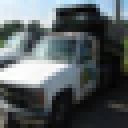
\includegraphics[width=11mm]{figures/flow/hard.png}};
\node[lab, anchor=south] at (34,60.6) {$x$};
\node[note, text width=39mm] at (4.3,37.2) {Preservation pool $\mathcal P$: correct images outside $\mathcal H$, with a class-balanced subset $\mathcal P_{\mathrm{causal}}\subseteq\mathcal P$};
\foreach \n/\px in {1/8.3, 2/16.3, 3/24.3}
  \node[thumb] at (\px,20.7) {\includegraphics[width=7mm]{figures/flow/pool\n.png}};
\node[stepnum] at (2,12.4) {2};
\node[note, text width=22mm] at (4.3,13.8) {Companions $x'$: the $n_{\mathrm{comp}}=5$ correct trucks outside $\mathcal H$ closest to $x$ in cosine similarity of pooled $T_0$ features};
\foreach \n/\d in {5/3.6, 4/2.7, 3/1.8, 2/0.9, 1/0}
  \node[thumb] at ({34+\d},{9.4-\d}) {\includegraphics[width=11mm]{figures/flow/companion\n.png}};

% teacher, activations, gradient and discrepancy
\node[draw, minimum width=10mm, minimum height=61mm, lab] (T) at (52,30.5) {Teacher\\$T_0$};
\draw[->] (39.5,55) -- (47,55);
\draw[->] (43.6,5.8) -- (47,5.8);
\node[draw, lab, minimum width=11mm, minimum height=6mm] (diff) at (67.5,37.5) {$|A-A'|$};
\node[circle, draw, inner sep=0pt, minimum size=4.4mm, font=\normalsize] (mul) at (79,37.5) {$\times$};
\draw[->] (57,57.5) -- node[above, lab, pos=0.25] {$G$} (79,57.5) -- (mul.north);
\draw[->] (57,51) -- node[above, lab, pos=0.4] {$A$} (67.5,51) -- (diff.north);
\draw[->] (57,19.5) -- node[above, lab, pos=0.4] {$A'$} (67.5,19.5) -- (diff.south);
\draw[->] (diff.east) -- node[above, lab] {$D$} (mul.west);
\node[block] at (85.8,37.5) {};
\node[lab, anchor=north] at (79,34.6) {$s=G\,D$};

% scoring: numbers give each channel's rank by the consensus score
\node[lab] at (98,49.5) {Scoring};
\netglyph{98}{31.5}
\foreach \i/\r in {1/3,2/1,3/5,4/2,5/4} \node[neuron, font=\sffamily\tiny] at ({98+(\i-3)*\gap},37.5) {\r};
\node[block] at (110.5,37.5) {};

% causal test: channel 1 (rank 3) is zeroed; channels 2 and 4 (ranks 1 and 2) were retained
\node[lab] at (123,49.5) {Causal test};
\netglyph{123}{31.5}
\foreach \i/\s in {1/2,2/1,3/0,4/1,5/0} {
  \ifcase\s \node[neuron] at ({123+(\i-3)*\gap},37.5) {};
  \or \node[neuron, fill=black!30] at ({123+(\i-3)*\gap},37.5) {};
  \or \node[neuron] (c) at ({123+(\i-3)*\gap},37.5) {};
      \draw (c.north west) -- (c.south east) (c.north east) -- (c.south west);
  \fi}

% (3) and (4) under the localization stages
\node[stepnum] at (61,15.6) {3};
\node[note, text width=36mm] at (63.3,17) {For each channel $a$ of the last two stages,\\[0.4mm]
  \hspace*{2mm}$G=\operatorname{mean}_{u,v}|\partial e/\partial A|$,\\[0.3mm]
  \hspace*{2mm}$D=\operatorname{mean}_{t,u,v}|A-A'_t|$,\\[0.3mm]
  \hspace*{2mm}$s=G\,D$,\\[0.4mm]
  where $e=z_r-z_y$ is the error margin against the strongest rival class $r$. Normalize $s$ by its stage mean, average it with equal class weight into $\overline s_a$, and keep $a$ as stable if $\widehat\pi_a\geq\pi_{\min}$, its share of bootstrap resamples that rank it in the top $\kappa$ fraction};
\node[stepnum] at (102,15.6) {4};
\node[note, text width=27.5mm] at (104.3,17) {Zero ($\times$) each stable $a$ in turn and retain it (grey) if\\[0.4mm]
  \hspace*{2mm}$\Delta_a^{\mathrm{tar}}>0$ and\\[0.3mm]
  \hspace*{2mm}$\Delta_a^{\mathrm{acc}}\geq-\eta_{\mathrm{acc}}$,\\[0.4mm]
  the changes in class-balanced hard-set margin and $\mathcal P_{\mathrm{causal}}$ accuracy. Rank the $J$ retained channels by $\Delta_a^{\mathrm{tar}}$};

% (5) masked update: bold edges produce and consume the edited channels (grey)
\node[block] at (137,52) {};
\node[lab] at (158,63.5) {Masked update};
\netglyph{158}{46}
\foreach \i/\s in {1/0,2/1,3/0,4/1,5/0} {
  \ifnum\s=1
    \foreach \h in {1,...,4} \draw[edit] ({158+(\h-2.5)*\gap},58) -- ({158+(\i-3)*\gap},52);
    \foreach \j in {1,...,4} \draw[edit] ({158+(\i-3)*\gap},52) -- ({158+(\j-2.5)*\gap},46);
  \fi}
\foreach \h in {1,...,4} \node[neuron] at ({158+(\h-2.5)*\gap},58) {};
\foreach \j in {1,...,4} \node[neuron] at ({158+(\j-2.5)*\gap},46) {};
\foreach \i/\s in {1/0,2/1,3/0,4/1,5/0} {
  \ifnum\s=1 \node[neuron, fill=black!30] at ({158+(\i-3)*\gap},52) {};
  \else \node[neuron] at ({158+(\i-3)*\gap},52) {}; \fi}
\node[stepnum] at (136.8,41.1) {5};
\node[note, text width=40mm] (upd) at (139.1,42.5) {For each feasible budget $n_{\mathrm{edit}}\le J$ and learning rate, update only $\Omega_{\mathrm{edit}}$, the parameters that produce, normalize or consume the top $n_{\mathrm{edit}}$ channels (bold), with the masked gradient $\mathbf 1_{\Omega_{\mathrm{edit}}}\odot\nabla_\theta\mathcal L_{\mathrm{rep}}$ of\\[0.5mm]
  \hspace*{2mm}$\mathcal L_{\mathrm{rep}}=\mathbb E_{\mathcal H}\mathcal L_{\mathrm{CE}}$\\[0.3mm]
  \hspace*{4mm}$+\lambda_{\mathrm P}\tau_{\mathrm r}^{2}\,\mathbb E_{\mathcal P}
   D_{\mathrm{KL}}(p_{\theta_0}^{(\tau_{\mathrm r})}\|\,p_\theta^{(\tau_{\mathrm r})})$\\[0.3mm]
  \hspace*{4mm}$+\lambda_{\mathrm F}\,\mathbb E_{\mathcal P}d_{\mathrm F}$};

% (6) selection and distillation
\draw[->] ([yshift=-1.2mm]159.5,0 |- upd.south) -- node[right, lab] {candidates} ++(0,-3.5) coordinate (c6);
\node[keep, draw, text width=38mm, align=flush left, inner sep=1.4mm, anchor=north] (sel) at (c6)
  {Keep the candidate with the highest validation $R_{\mathrm{tar}}$ among those with\\[0.4mm]
   \hspace*{2mm}$R_{\mathrm{tar}}(T_\theta)>R_{\mathrm{tar}}(T_0)$ and\\[0.3mm]
   \hspace*{2mm}$\operatorname{Acc}(T_\theta)\geq\operatorname{Acc}(T_0)-\eta_{\mathrm{sel}}$;\\[0.4mm]
   if there is none, keep $T_0$};
\node[stepnum] at ([yshift=-3.2mm]136.8,0 |- sel.north) {6};
\draw[->] (sel.south) -- ++(0,-3.5);
\node[keep, draw, rounded corners=2mm, lab, text width=38mm, align=flush center, anchor=north, inner sep=1.2mm]
  at ([yshift=-3.5mm]sel.south) {Distill the student $S$ from the returned teacher $T$ with\\[0.4mm]
  $\mathcal L_{\mathrm{KD}}=\mathbb E\bigl[\alpha\mathcal L_{\mathrm{CE}}$\\[0.3mm]
  $+(1-\alpha)\tau^{2}D_{\mathrm{KL}}(p_T^{(\tau)}\|\,p_S^{(\tau)})\bigr]$};
\end{tikzpicture}
\vspace{-4pt}
\caption{Overview of the teacher repair. The example is a CIFAR-10 hard
image at $\rho=10$, a truck that $T_0$ labels an automobile, with correctly
classified trucks as its companions.}
\label{fig:repair-flow}
\vspace{-6pt}
\end{figure*}

\subsection{Notation and objective}

Let $\mathcal{D}_{\mathrm{rep}}=\{(x_i,y_i)\}_{i=1}^{N}$ be
a labeled pool of $N$ images with labels in $\mathcal{Y}$,
where $|\mathcal{Y}|\geq2$.
The nonempty set
$\mathcal{C}_{\mathrm{tar}}\subseteq\mathcal{Y}$ specifies the
classes whose teacher behavior we intend to repair. Each
target class must have at least one image in the pool.
The original teacher $T_0=f_{\theta_0}$ remains fixed.
The candidate $T_\theta=f_\theta$ has the same architecture
and starts from $\theta_0$, where
$\theta\in\mathbb{R}^{d_\theta}$ contains $d_\theta$ scalar
parameters. Table~\ref{S-tab:notation} in the supplementary material
lists the main symbols.

For a teacher $T=f_\theta$, the logits are denoted by
$z_\theta(x)=z_T(x)$, following the model notation of
Eq.~\eqref{eq:softmax-temperature}, and its
probability vector $p_\theta^{(\tau)}(x)=p_T^{(\tau)}(x)$ has
components
\begin{equation}
\label{eq:repair-probabilities}
p_{\theta,c}^{(\tau)}(x)=
\frac{\exp(z_{\theta,c}(x)/\tau)}
{\sum_{r\in\mathcal{Y}}\exp(z_{\theta,r}(x)/\tau)},
\qquad c\in\mathcal{Y},
\end{equation}
where $\tau>0$. We omit the superscript when $\tau=1$.

We inspect a nonempty set $\mathcal{L}_{\mathrm{loc}}$ of
later convolutional stages in the teacher. At stage $\ell$,
the feature map
$A_\theta^{(\ell)}(x)\in
\mathbb{R}^{K_\ell\times U_\ell\times V_\ell}$
has $K_\ell$ channels and spatial dimensions $U_\ell,V_\ell$.
Its entries are $A_{\theta,k,u,v}^{(\ell)}(x)$, where
$1\leq k\leq K_\ell$, $1\leq u\leq U_\ell$, and
$1\leq v\leq V_\ell$. Throughout this section, sums over
$u,v$ cover these spatial positions, and a colon in the
channel index denotes the full channel vector.
The candidate channel set is
\begin{equation}
\mathcal{A}_{\mathrm{loc}}=
\{(\ell,k):\ell\in\mathcal{L}_{\mathrm{loc}},
                  \ 1\leq k\leq K_\ell\}.
\end{equation}
We write $a=(\ell,k)$ for a channel and use $\epsilon>0$
to keep normalization denominators away from zero.

For an image with true label $y_i$, define the strongest
competing class under $T_0$ and its error margin by
\begin{equation}
\label{eq:repair-error-margin}
\begin{aligned}
r_i&=\argmax_{r\in\mathcal{Y}\setminus\{y_i\}}
                 z_{\theta_0,r}(x_i),\\
e_i&=z_{\theta_0,r_i}(x_i)-z_{\theta_0,y_i}(x_i).
\end{aligned}
\end{equation}
A positive $e_i$ means the competitor wins. A negative value
close to zero indicates a correct decision with little
separation. Predictions and rankings use a fixed ordering
to resolve exact ties. The mechanism finds hard images,
localizes associated channels, checks them by intervention,
updates only parameters connected to the selected channels,
and selects one candidate on validation data
(Fig.~\ref{fig:repair-flow}). This
localize-then-edit design follows AI-Lancet~\cite{zhao2021ailancet};
Section~\ref{sec:research-gap} describes how the two differ.
\vspace{-5pt}
\subsection{Step 1: Construct hard and preservation sets}

Let $\widehat y_i=\argmax_{r\in\mathcal{Y}}
z_{\theta_0,r}(x_i)$ be the original teacher's prediction.
For each class $c$, define the image indices
$I_c=\{i\in\{1,\ldots,N\}:y_i=c\}$ and the misclassified
indices $M_c=\{i\in I_c:\widehat y_i\ne c\}$.
On each unaugmented image, compute the true-class negative
log-likelihood (NLL)
$\nu_i=-\log p_{\theta_0,y_i}(x_i)$.

For each target class, the hard index set $H_c$ contains
all mistakes. We add the highest-NLL correctly classified
images until it reaches a quota
$n_c^{\mathrm{hard}}=\lceil\xi|I_c|\rceil$, where
$\xi\in(0,1]$ is the requested fraction:
\begin{equation}
\label{eq:repair-hard-set}
\begin{aligned}
H_c&=M_c\cup
\operatorname{TopNLL}_{(n_c^{\mathrm{hard}}-|M_c|)_+}
       (I_c\setminus M_c),\\
\mathcal{H}&=\{(x_i,y_i):i\in
          \bigcup_{c\in\mathcal{C}_{\mathrm{tar}}}H_c\}.
\end{aligned}
\end{equation}
Here $\operatorname{TopNLL}_j$ returns the $j$ indices with
largest $\nu_i$, returns the empty set when $j=0$, and
$(v)_+=\max(v,0)$. All mistakes remain even when they exceed
the quota. The added images make the repair attend to
uncertain correct decisions as well as outright mistakes.
Thus $H_c$ contains indices, while $\mathcal{H}$ contains
the corresponding labeled examples.

The preservation pool contains correctly classified examples
outside the hard set:
\begin{equation}
\label{eq:repair-preservation-set}
\mathcal{P}=
\{(x_i,y_i)\in\mathcal{D}_{\mathrm{rep}}\setminus\mathcal{H}:
  \widehat y_i=y_i\}.
\end{equation}
It can include images from target classes. A smaller,
nonempty subset $\mathcal{P}_{\mathrm{causal}}\subseteq\mathcal{P}$
contains the same number of examples from each represented
class and is used in Step 4. Repair requires a nonempty
preservation pool. Both sets are constructed from $T_0$
and remain fixed.

Let $q_{\mathcal H}$ and $q_{\mathcal P}$ be distributions
over labeled examples in $\mathcal H$ and $\mathcal P$. Each first
chooses a represented class uniformly, then an example
uniformly within that class. They therefore give each
represented class equal weight.

\vspace{-5pt}
\subsection{Step 2: Find successful companions}

A hard image is compared with images of the same class that
the teacher already recognizes correctly. Let
$\ell_{\mathrm{last}}\in\mathcal{L}_{\mathrm{loc}}$ be the
deepest localized stage. Globally average-pool its feature
map and normalize the resulting vector:
\begin{equation}
\label{eq:repair-embedding}
\begin{aligned}
v_i&=\operatorname{GAP}
 \bigl(A_{\theta_0}^{(\ell_{\mathrm{last}})}(x_i)\bigr),\\
h_i&=v_i/\max(\|v_i\|_2,\epsilon).
\end{aligned}
\end{equation}
Here $\operatorname{GAP}$ averages each channel over spatial
positions. Let $n_{\mathrm{comp}}$ be a positive integer
specifying the requested number of companions.
For each $i\in H_c$, rank the eligible indices
$(I_c\setminus M_c)\setminus H_c$ by decreasing
$h_i^\top h_j$. For nonzero embeddings above the numerical
floor, this inner product is their cosine similarity.
The first $n_{\mathrm{comp}}$ indices form the companion
list $\mathcal{N}_i=(j_{i,1},\ldots,j_{i,n_{\mathrm{comp}}})$.

When sparse fallback is enabled and too few eligible
images exist, we instead rank the other same-class indices
$I_c\setminus\{i\}$. These fallback images need not be
correctly classified. If fewer than $n_{\mathrm{comp}}$
remain, the ranked list is repeated to fill the requested
length. Thus $\mathcal{N}_i$ is a list of indices and may
contain repetitions. If no other same-class image exists,
we take $\mathcal{N}_i$ to be empty and use gradient
sensitivity alone in Step 3. Without fallback, the procedure
requires enough eligible companions for every hard image.

For example, if $T_0$ labels a truck as an automobile,
the preferred companions are trucks that $T_0$
labels correctly. The comparison asks which channels differ
between these cases and can affect the automobile-versus-truck
logit gap.

\vspace{-5pt}
\subsection{Step 3: Score and stabilize channels}

For each hard image index $i$ and channel $(\ell,k)$, compute
the sensitivity of the error margin to that channel:
\begin{equation}
\label{eq:repair-sensitivity}
G_{i,\ell,k}=
\frac{1}{U_\ell V_\ell}
\sum_{u,v}
\left|
\frac{\partial e_i}
{\partial A_{\theta_0,k,u,v}^{(\ell)}(x_i)}
\right|.
\end{equation}
For a nonempty companion list, also compute the mean
activation difference:
\begin{equation}
\label{eq:repair-discrepancy}
D_{i,\ell,k}=
\frac{\sum_{t=1}^{n_{\mathrm{comp}}}\sum_{u,v}
\left|
A_{\theta_0,k,u,v}^{(\ell)}(x_i)-
A_{\theta_0,k,u,v}^{(\ell)}(x_{j_{i,t}})
\right|}
{n_{\mathrm{comp}}U_\ell V_\ell}.
\end{equation}
Large $G_{i,\ell,k}$ means a local change in the channel
could change the error margin. Large $D_{i,\ell,k}$ means
its activation differs from its same-class companions;
under the preferred selection rule, these are examples
the teacher gets right. Their product favors channels
satisfying both conditions.

Set $s_{i,\ell,k}=G_{i,\ell,k}D_{i,\ell,k}$ when
$\mathcal N_i$ is nonempty. When it is empty, set
$s_{i,\ell,k}=G_{i,\ell,k}$ without computing $D_{i,\ell,k}$.
Normalize each image's scores by the mean score in its stage:
\begin{equation}
\label{eq:repair-channel-score}
\widetilde{s}_{i,\ell,k}=
\frac{s_{i,\ell,k}}
{\max\{K_\ell^{-1}\sum_{k'=1}^{K_\ell}
s_{i,\ell,k'},\epsilon\}}.
\end{equation}
For $a=(\ell,k)$, write
$\widetilde{s}_{i,a}=\widetilde{s}_{i,\ell,k}$.
Average first within each target class, then across classes:
\begin{equation}
\label{eq:repair-consensus}
\overline{s}_a=
\frac{1}{|\mathcal C_{\mathrm{tar}}|}
\sum_{c\in\mathcal C_{\mathrm{tar}}}
\frac{1}{|H_c|}\sum_{i\in H_c}\widetilde{s}_{i,a}.
\end{equation}
This gives each target class equal weight.

To test ranking stability, draw $B_{\mathrm{boot}}$ stratified
bootstrap resamples, where $B_{\mathrm{boot}}$ is a positive
integer. Each resample draws $|H_c|$ indices with replacement
from every $H_c$ and recomputes Eq.~\eqref{eq:repair-consensus}.
Let $\overline{s}_a^{(\beta)}$ be the score in resample
$\beta\in\{1,\ldots,B_{\mathrm{boot}}\}$.
For a retained fraction $\kappa\in(0,1]$, let
$\mathcal A_{\kappa}^{(\beta)}$ contain the
$\lceil\kappa|\mathcal A_{\mathrm{loc}}|\rceil$
highest-scoring channels in that resample. Define
\begin{equation}
\label{eq:repair-stability}
\begin{aligned}
\widehat{\pi}_a
&=\frac{1}{B_{\mathrm{boot}}}
  \sum_{\beta=1}^{B_{\mathrm{boot}}}
  \mathbf{1}[a\in\mathcal A_{\kappa}^{(\beta)}],\\
\mathcal A_{\mathrm{stable}}
&=\{a\in\mathcal A_{\mathrm{loc}}:
                \widehat{\pi}_a\geq\pi_{\min}\},
\end{aligned}
\end{equation}
where $\mathbf{1}[\cdot]$ is one when its condition holds
and zero otherwise, and $\pi_{\min}\in[0,1]$ is the minimum
selection frequency. We order stable channels by
$\overline{s}_a$. Repeated selection identifies an association
between a channel and the hard-image behavior. To determine
whether suppressing that channel helps the hard images while
preserving other decisions, Step 4 tests it by intervention.

\vspace{-5pt}
\subsection{Step 4: Test channels by temporary intervention}

For each $a\in\mathcal A_{\mathrm{stable}}$, let $T_0^{-a}$
denote the original teacher with that channel's entire
output temporarily set to zero. For any teacher $T$, define
the true-class margin and its class-balanced mean by
\begin{equation}
\label{eq:repair-true-margin}
\begin{aligned}
m(T;x,y)&=z_{T,y}(x)-
 \max_{r\in\mathcal Y\setminus\{y\}}z_{T,r}(x),\\
\overline m_{\mathcal H}(T)
&=\mathbb E_{(x,y)\sim q_{\mathcal H}}m(T;x,y).
\end{aligned}
\end{equation}
In particular, $m(T_0;x_i,y_i)=-e_i$, so a larger true-class
margin corresponds to a smaller error margin.

Let $\operatorname{Acc}_{\mathrm{causal}}(T)$ denote the
fraction of correct predictions on
$\mathcal P_{\mathrm{causal}}$. Let
$\operatorname{NLL}_{\mathrm{causal}}(T)$ denote the mean
$-\log p_{T,y}^{(1)}(x)$ over that same pool.
For a causal guardrail $\eta_{\mathrm{acc}}\in[0,1]$, the largest
accuracy drop allowed on $\mathcal P_{\mathrm{causal}}$, compute
\begin{equation}
\label{eq:repair-causal-gate}
\begin{aligned}
\Delta_a^{\mathrm{tar}}
&=\overline m_{\mathcal H}(T_0^{-a})
 -\overline m_{\mathcal H}(T_0),\\
\Delta_a^{\mathrm{acc}}
&=\operatorname{Acc}_{\mathrm{causal}}(T_0^{-a})
 -\operatorname{Acc}_{\mathrm{causal}}(T_0).
\end{aligned}
\end{equation}
Retain the channel when $\Delta_a^{\mathrm{tar}}>0$ and
$\Delta_a^{\mathrm{acc}}\geq-\eta_{\mathrm{acc}}$.
The first condition asks whether suppressing the channel
improves target margins. The second limits the loss of
preservation accuracy. Among channels satisfying both,
we prefer the largest target-margin gain. Ties are resolved
by lower $\operatorname{NLL}_{\mathrm{causal}}(T_0^{-a})$.
After each intervention, we restore the channel output.
Step 5 therefore begins from the intact original teacher.

\vspace{-5pt}
\subsection{Step 5: Update only selected parameters}

Let $n_{\mathrm{edit}}$ be a positive integer specifying the
requested number of channels to edit. Write the $J$ channels
that passed Step 4 in rank order as
$(a_{(1)},\ldots,a_{(J)})$. A budget is feasible only when
$n_{\mathrm{edit}}\leq J$; an infeasible budget produces no
repair candidate. For a feasible budget, define
\begin{equation}
\label{eq:repair-edit-support}
\begin{aligned}
\mathcal A_{\mathrm{edit}}
&=\{a_{(r)}:1\leq r\leq n_{\mathrm{edit}}\},\\
\Omega_{\mathrm{edit}}
&=\bigcup_{a\in\mathcal A_{\mathrm{edit}}}\Omega(a).
\end{aligned}
\end{equation}
Here $\Omega(a)\subseteq\{1,\ldots,d_\theta\}$ contains the
parameter coordinates of channel $a$'s producing
convolutional filter, normalization scale and bias
parameters where present, and corresponding weights in
direct consumers. Initialize the candidate with
$\theta=\theta_0$ and hold every coordinate outside
$\Omega_{\mathrm{edit}}$ fixed.

For the masked updates, let $\widetilde q_{\mathcal H}$ and
$\widetilde q_{\mathcal P}$ be the distributions obtained
by applying the configured label-preserving augmentation to
examples drawn from $q_{\mathcal H}$ and $q_{\mathcal P}$.
The candidate and original teacher receive the same
augmented view of each preservation example. Diagnosis and
channel screening use the unaugmented images.

The repair objective has one term for hard examples and two
for preservation examples. Let $\tau_{\mathrm r}>0$ be the
repair temperature and $\lambda_{\mathrm P},\lambda_{\mathrm F}
\geq0$ the weights for output and feature preservation:
\begin{equation}
\label{eq:teacher-repair-loss}
\begin{aligned}
\mathcal L_{\mathrm{rep}}(\theta)
={}&\mathbb E_{(x,y)\sim\widetilde q_{\mathcal H}}
  \mathcal L_{\mathrm{CE}}(y,p_\theta(x))\\
&+\lambda_{\mathrm P}\tau_{\mathrm r}^{2}
\mathbb E_{(x,y)\sim\widetilde q_{\mathcal P}}
 D_{\mathrm{KL}}\!\left(
 p_{\theta_0}^{(\tau_{\mathrm r})}(x)
 \,\middle\|\,p_\theta^{(\tau_{\mathrm r})}(x)\right)\\
&+\lambda_{\mathrm F}
\mathbb E_{(x,y)\sim\widetilde q_{\mathcal P}}
 d_{\mathrm F}(T_\theta,T_0;x).
\end{aligned}
\end{equation}
The cross-entropy term pushes the teacher toward correct
labels on hard images. The KL term keeps its output
distribution close to $T_0$ on preservation images.

The feature term restrains changes to internal
representations. At each spatial position, normalize the
channel vector with a denominator floor:
\begin{equation}
\label{eq:repair-feature-normalization}
\widehat A_\theta^{(\ell)}(x)_{:,u,v}
=
\frac{A_\theta^{(\ell)}(x)_{:,u,v}}
{\max\{\|A_\theta^{(\ell)}(x)_{:,u,v}\|_2,\epsilon\}}.
\end{equation}
This definition also handles a zero vector. The feature
distance is
\begin{equation}
\label{eq:repair-feature-loss}
\begin{aligned}
d_{\mathrm F}(T_\theta,T_0;x)
={}&\frac{1}{|\mathcal L_{\mathrm{loc}}|}
\sum_{\ell\in\mathcal L_{\mathrm{loc}}}
\frac{1}{U_\ell V_\ell}\\
&\cdot\sum_{u,v}
\left\|
\widehat A_\theta^{(\ell)}(x)_{:,u,v}
-\widehat A_{\theta_0}^{(\ell)}(x)_{:,u,v}
\right\|_2^2.
\end{aligned}
\end{equation}
Each update uses the masked gradient
$\mathbf{1}_{\Omega_{\mathrm{edit}}}\odot
\nabla_\theta\mathcal L_{\mathrm{rep}}$.
Here $\mathbf{1}_{\Omega_{\mathrm{edit}}}\in\{0,1\}^{d_\theta}$
has a one exactly at editable coordinates, and $\odot$
denotes elementwise multiplication.
The optimizer uses momentum SGD with zero weight decay.
Normalization running statistics and all other model buffers
stay fixed throughout the updates. After optimization,
the implementation verifies that every coordinate outside
$\Omega_{\mathrm{edit}}$ and every buffer is identical to
$T_0$. The result is a teacher repaired within the selected
parameter support.

\vspace{-5pt}
\subsection{Step 6: Select a candidate on validation data}
\label{sec:repair-selection}

Steps 1--4 run once for each teacher. Step 5 then trains one candidate
for each feasible channel budget in a grid and each learning rate, and
this step chooses among them on the validation set
$\mathcal D_{\mathrm{val}}$ (Section~\ref{sec:datasets}). Let
$\operatorname{Acc}$, $R_{\mathrm{tar}}$ and
$\operatorname{NLL}_{\mathrm{tar}}$ be the overall accuracy,
target-class recall and target-balanced NLL of
Section~\ref{sec:evaluation-metrics} on
$\mathcal D_{\mathrm{val}}$. For a selection guardrail
$\eta_{\mathrm{sel}}\in[0,1]$, a candidate $T_\theta$ is acceptable
when
\begin{equation}
\label{eq:repair-selection}
R_{\mathrm{tar}}(T_\theta)>R_{\mathrm{tar}}(T_0)
\;\;\text{and}\;\;
\operatorname{Acc}(T_\theta)\geq\operatorname{Acc}(T_0)-\eta_{\mathrm{sel}}.
\end{equation}
Among acceptable candidates, we select the one with the highest
$R_{\mathrm{tar}}$, breaking ties by lower
$\operatorname{NLL}_{\mathrm{tar}}$, then by the smaller budget and then
by the lower learning rate. If no budget is feasible or no candidate is
acceptable, the procedure returns $T_0$ unchanged.

\vspace{-5pt}
\section{Experimental Design}
\label{sec:experimental-design}

\subsection{Datasets}
\label{sec:datasets}

We evaluate on thirteen image-classification benchmarks chosen to span
visual domains, class counts and native resolutions. Five contain natural
images: CIFAR-10 and CIFAR-100~\cite{krizhevsky2009learning},
CINIC-10~\cite{darlow2018cinic}, STL-10~\cite{coates2011analysis} and
Caltech-101~\cite{feifei2004learning}. Four come from other visual
domains: street-view house numbers (SVHN~\cite{netzer2011reading}),
clothing (Fashion-MNIST~\cite{xiao2017fashion}), traffic signs
(GTSRB~\cite{stallkamp2012man}) and satellite imagery
(EuroSAT~\cite{helber2019eurosat}). The remaining four are medical, taken
from MedMNIST~v2~\cite{yang2023medmnist}: colon pathology (PathMNIST),
blood-cell microscopy (BloodMNIST), dermatoscopy (DermaMNIST) and
abdominal computed tomography (OrganAMNIST). The number of classes $C$
ranges from 7 to 101. The supplementary material gives the full
experimental settings; its sections and tables carry the prefix S.

Each dataset has disjoint training, validation and test sets,
$\mathcal{D}_{\mathrm{tr}}$, $\mathcal{D}_{\mathrm{val}}$ and
$\mathcal{D}_{\mathrm{test}}$. Every teacher and student is trained on
$\mathcal{D}_{\mathrm{tr}}$, which also serves as the repair pool
$\mathcal{D}_{\mathrm{rep}}$, whereas $\mathcal{D}_{\mathrm{val}}$ selects
checkpoints and repair candidates, and $\mathcal{D}_{\mathrm{test}}$
stays sealed until the teacher and every student checkpoint of a run
have been fixed. We use the official splits where they exist and
otherwise hold out stratified parts of the training images.
Section~\ref{S-app:datasets} gives the sizes, splits and classes of every
dataset (Tables~\ref{S-tab:datasets} and~\ref{S-tab:dataset-classes}).

\textbf{Imbalance profiles.} Each dataset is used at four nominal
imbalance factors, $\rho\in\{1,10,50,100\}$, giving 52 dataset--profile
settings. Adapting the exponential long-tail schedule
of~\cite{cui2019class}, class $c\in\{0,\ldots,C-1\}$ keeps
\begin{equation}
\label{eq:imbalance-profile}
n_c=\max\!\left\{1,\operatorname{round}\!\left(\widetilde n_c\,\rho^{-c/(C-1)}\right)\right\}
\end{equation}
of its $\widetilde n_c$ available images, where classes follow the
dataset's native label order. Class $0$ keeps all of its images, class
$C-1$ about a $1/\rho$ fraction, and every class at least one image. Both $\mathcal{D}_{\mathrm{tr}}$ and
$\mathcal{D}_{\mathrm{val}}$ are resampled this way;
$\mathcal{D}_{\mathrm{test}}$ is not, so every model is evaluated on the
dataset's native test distribution. At $\rho=1$ no image is removed, and
each dataset keeps its native imbalance.

\textbf{Target classes.} For $\rho>1$, the target set
$\mathcal{C}_{\mathrm{tar}}$ contains the $\lceil C/2\rceil$ classes with
the fewest training images, ties broken by label. For $\rho=1$ it contains
all classes, so the repair addresses errors of the whole model.

\textbf{Preprocessing.} All images are used as $32\times32$ RGB tensors
normalized per channel. Training images are randomly cropped and are
flipped horizontally only where mirroring preserves the label, and
evaluation images are never augmented (Section~\ref{S-app:datasets}).

\vspace{-5pt}
\subsection{Models and Training Parameters}
\label{sec:training-parameters}

\textbf{Models.} The design uses three teachers, CNN-T, ResNet-18 and
ResNet-34, and one student, CNN-S, all taking $32\times32$ RGB inputs.
CNN-T and CNN-S share one design with three stages, each of two
$3\times3$ convolutions with batch normalization and ReLU followed by
$2\times2$ max pooling, and a linear classifier on the feature map
average-pooled to $2\times2$; CNN-S halves CNN-T's width at every stage.
ResNet-18 and ResNet-34~\cite{he2016deep} stack basic residual blocks in
four stages behind a $3\times3$, stride-one stem. The repair searches the
output channels of each teacher's last two stages, 192 in CNN-T and 768
in each ResNet. Because every teacher is distilled into CNN-S, the
teacher sets the capacity gap. CNN-T has 3.9 times the parameters and
FLOPs of CNN-S, whereas ResNet-18 has 149 times the parameters and 56
times the FLOPs, and ResNet-34 284 and 117 times
(Table~\ref{S-tab:architectures}), a gap more than an order of magnitude
wider than that of the CNN pair.

\textbf{Teacher--student pairings.} For each teacher and each of the 52
settings, CNN-S is distilled first from the original teacher and then
from the output of the teacher-repair procedure, with matched student
initializations and training conditions. If no repair candidate passes
selection, the procedure returns the original teacher unchanged, and its
original-teacher student serves as the no-change outcome. The repair
effect is then zero, and the setting remains in the aggregate
comparison. The alternative KD losses use the original teacher.

\textbf{Student choice.} The student is the model that is deployed, so
its size is set by the target hardware, whereas the teacher can be
chosen freely. We therefore distill every teacher into the same student,
whose architecture, training recipe, data, seeds and initial weights are
identical across teachers, so differences in transfer between teachers
are attributable to the teacher. The cost of this choice is that the
capacity gap grows with the teacher, into a regime in which distillation
is known to weaken~\cite{cho2019efficacy}.

\textbf{Training and distillation.} A separate teacher is trained from
scratch with cross-entropy for each dataset--profile setting and teacher
architecture, using SGD with cosine decay, and teacher and student
checkpoints are chosen by validation accuracy
(Table~\ref{S-tab:training-parameters}). CNN-S is trained with the same
recipe whichever teacher it learns from, from three initializations per
condition that are paired across teacher conditions and KD losses. The
teacher is frozen while the student trains, and with both the original
and the repaired teacher the student uses the classical KD objective of
Eq.~\eqref{eq:kd}. In epoch $e$, counting from one, the implemented
per-example loss is
\begin{equation}
\label{eq:experimental-kd-loss}
\begin{aligned}
\mathcal L_{\mathrm{student}}^{(e)}={}&
0.5\,\mathcal L_{\mathrm{CE}}\!\left(y,p_S^{(1)}(x)\right)\\
&+0.5\,w_e\,4^2 D_{\mathrm{KL}}\!\left(
p_T^{(4)}(x)\,\middle\|\,p_S^{(4)}(x)\right),\\
w_e={}&\min\{e/5,1\},
\end{aligned}
\end{equation}
so the response term grows over the first five epochs while the
hard-label coefficient stays fixed.

\textbf{Teacher repair.} Localization examines the last two
convolutional stages of each teacher with $\xi=0.2$,
$n_{\mathrm{comp}}=5$, $B_{\mathrm{boot}}=20$, $\kappa=0.25$ and
$\pi_{\min}=0.7$, and both guardrails are
$\eta_{\mathrm{acc}}=\eta_{\mathrm{sel}}=0.005$;
Table~\ref{S-tab:repair-parameters} lists the remaining settings.
Candidates edit two, four or eight channels, each with learning rates
0.001 and 0.005. This grid is the same for every teacher, so that
architecture is the only factor that changes, but because each ResNet's
searched stages hold 768 channels against 192 in CNN-T, it edits
1.0--4.2\% of CNN-T's searched channels and only 0.26--1.04\% of a
ResNet's. We therefore also repaired both ResNet teachers with a
prespecified scaled grid, $n_{\mathrm{edit}}\in\{8,16,32\}$, which
restores the CNN-T fractions and reuses the same teachers,
original-teacher students, localization, optimization and selection
gate; its results are reported separately.

\textbf{Alternative distillation losses.} We compare teacher repair with
LoCa~\cite{yang2024loca}, DKD~\cite{zhao2022decoupled} and
RLD~\cite{sun2025knowledge}, trained from the original teacher with the
same temperature, warm-up, student optimization and training examples as
classical KD. At the published weights, the median response term of DKD
and RLD is 24--28 and 13--22 times the cross-entropy, against 5--8 times
for classical KD, so we also train each at a lower response weight that
matches the ratio of classical KD. That weight was fixed for each teacher
from training histories alone, before any test evaluation
(Section~\ref{S-app:loss-settings}).

\vspace{-5pt}
\subsection{Evaluation Metrics and Comparison Protocol}
\label{sec:evaluation-metrics}

Once training and validation have fixed the teacher and student
checkpoints, we evaluate them on the test set. For a model $M$, let
$\operatorname{Acc}(M)$ be the fraction of test images that it classifies
correctly and $R_c(M)$ the fraction of class-$c$ test images that it
assigns to class $c$, the recall of class $c$. Because repair focuses on
$\mathcal C_{\mathrm{tar}}$, our primary class-sensitive measure averages
recall over those classes:
\begin{equation}
\label{eq:target-recall}
R_{\mathrm{tar}}(M)=\frac{1}{|\mathcal C_{\mathrm{tar}}|}
\sum_{c\in\mathcal C_{\mathrm{tar}}}R_c(M).
\end{equation}
At $\rho=1$, the target set contains every class, and
$R_{\mathrm{tar}}$ is therefore macro recall, also called balanced
accuracy. We also report
macro-F1, the negative log-likelihood (NLL) of the true class, the
multiclass Brier score, the expected calibration error over 15 bins
(ECE$_{15}$), the area under the risk--coverage curve (AURC) and
selective accuracy at 80\% and 90\% coverage, all defined in
Section~\ref{S-supp:metrics}. The target-balanced NLL,
$\operatorname{NLL}_{\mathrm{tar}}$, averages the true-class NLL within
each target class and then across target classes, so it weights target
classes equally; it also breaks ties in repair selection.

We compare each selected repair with its original teacher using
accuracy and $R_{\mathrm{tar}}$. The central comparison then asks
whether the change reaches the student. For each teacher--student
pairing and student initialization, we subtract the original-teacher
student's accuracy and target recall from the corresponding scores of
the student trained with the repair procedure's output, making
improvements positive. We then average these differences over the
three matched initializations of each setting. We call the transfer
successful if mean target recall rises by at least one percentage
point, at least two seeds show a positive recall change, and mean
accuracy falls by no more than 0.5 percentage points. LoCa, DKD and
RLD students are evaluated on the same images with matched
initializations.

To include settings where repair fails selection, we retain all 52
settings in each pairing's summary. In a no-change setting, the
original student's result is reused, giving zero difference in both
metrics. We also report results for settings that selected
a repair. To test whether the per-setting differences, each averaged
over the three initializations, are centered on zero, we apply a
two-sided Wilcoxon signed-rank test; settings with a zero difference,
including every no-change setting, are dropped, as the test prescribes.

\FloatBarrier
\vspace{-5pt}
\section{Experimental Results and Analysis}
\label{sec:results}

This section measures how teacher repair changes the student. We
express differences between a repaired-teacher condition and its
matched original-teacher condition in percentage points (pp) for
accuracy, recall, F1 and ECE, and we test them across settings with the
Wilcoxon signed-rank test of Section~\ref{sec:evaluation-metrics}. The
student is CNN-S throughout, and every comparison covers all 13
datasets at four imbalance factors (52 settings): CNN-T, ResNet-18 and
ResNet-34 with the fixed channel grid, the two ResNet teachers with the
scaled grid, and the alternative losses for each teacher.
Section~\ref{sec:overall-performance} first gives the overall change in
the student for each teacher and channel budget, and
Section~\ref{sec:sota-comparison} compares teacher repair with
classical KD and three recent losses, LoCa, DKD and RLD.
Section~\ref{sec:teacher-student-changes} then follows the change from
each repaired teacher to its student in the settings that selected a
repair, and Section~\ref{sec:teacher-architecture} relates the repair
decisions to the teacher's architecture and channel budget.

\vspace{-5pt}
\subsection{Overall Performance by Teacher}
\label{sec:overall-performance}
\suppressfloats[t]

Table~\ref{tab:overall-pair-results} shows how teacher repair changes
the CNN-S student for each teacher and channel budget. Each entry
subtracts the student distilled from the original teacher from the
student distilled from the repaired teacher, and the two students share
their initialization, data and schedule. We average these differences
over the three seeds and then across settings. In the all-settings
columns, a setting where no repair was selected counts as zero,
whereas the selected-only columns average only the settings that
selected a repair. Selected gives the number of such settings, and
Transfer counts the repairs that meet the rule in
Section~\ref{sec:evaluation-metrics}. Because the Wilcoxon test drops
zero differences, the stars on the all-settings columns hold for the
selected-only columns as well. Section~\ref{S-app:dataset-student-outcomes}
gives dataset-level outcome counts under both budgets.

\begin{table}[htb]
\caption{Change in CNN-S performance (pp) when the teacher is
repaired, from its performance when the teacher is not repaired. Stars
mark significant changes in the Wilcoxon signed-rank test
($^{*}p<0.05$, $^{**}p<0.01$, $^{***}p<0.001$).}
\label{tab:overall-pair-results}
\centering
\footnotesize
\setlength{\tabcolsep}{3pt}
\renewcommand{\arraystretch}{1.1}
\vspace{-3pt}
\begin{tabular}{@{}lcrrrrc@{}}
\toprule
& & \multicolumn{2}{c}{All settings} & \multicolumn{2}{c}{Selected only} & \\
\cmidrule(lr){3-4}\cmidrule(lr){5-6}
Teacher & Selected & $\Delta\mathrm{Acc}$ & $\Delta R_{\mathrm{tar}}$
& $\Delta\mathrm{Acc}$ & $\Delta R_{\mathrm{tar}}$ & Transfer \\
\midrule
\multicolumn{7}{@{}l}{\textit{Channel budget 2/4/8}} \\
CNN-T & 23/52 & $+0.23^{**}$ & $+0.69^{***}$ & $+0.51$ & $+1.55$ & 10/23 \\
ResNet-18 & 18/52 & $+0.05$ & $+0.20$ & $+0.14$ & $+0.57$ & 5/18 \\
ResNet-34 & 21/52 & $+0.03$ & $+0.16$ & $+0.08$ & $+0.41$ & 4/21 \\
\midrule
\multicolumn{7}{@{}l}{\textit{Channel budget 8/16/32}} \\
ResNet-18 & 17/52 & $+0.05$ & $+0.31^{*}$ & $+0.14$ & $+0.95$ & 4/17 \\
ResNet-34 & 18/52 & $+0.13^{*}$ & $+0.21^{*}$ & $+0.38$ & $+0.62$ & 5/18 \\
\bottomrule
\end{tabular}
\vspace{-3pt}
\end{table}

Teacher repair helped the student most when the teacher was CNN-T. It
raised both accuracy and target recall significantly over all 52
settings, and ten of its 23 repairs met the transfer rule. With the
ResNet teachers the gains were much smaller. Under the 2/4/8 budget
neither ResNet teacher changed the student significantly. Under the
8/16/32 budget both gave small but significant recall gains, and
ResNet-34 raised accuracy significantly as well. These gains were still
smaller than with CNN-T, however, and did not differ significantly
from those of the 2/4/8 budget
(Section~\ref{sec:teacher-architecture}).

\FloatBarrier
\vspace{-5pt}
\subsection{Comparison with State-of-the-Art Methods}
\label{sec:sota-comparison}
\suppressfloats[t]

Table~\ref{tab:loss-results} compares teacher repair with classical KD
and with three recent response-based methods,
LoCa~\cite{yang2024loca}, DKD~\cite{zhao2022decoupled} and
RLD~\cite{sun2025knowledge}. We train these methods from the original
teacher, and we also train DKD and RLD at the lower response weights
described in Section~\ref{sec:training-parameters}. Each entry is the
CNN-S test score averaged over three seeds and then across all 52
settings. Where no repair was selected, teacher repair keeps the
original teacher and its entry uses the classical-KD student, so every
method is compared over the same settings. Significance comes from the
paired Wilcoxon signed-rank test in
Section~\ref{sec:evaluation-metrics}.

\begin{table}[htb]
\caption{CNN-S accuracy and target recall (\%) for each method and
teacher, averaged over all 52 settings. Bold marks the best result in
each column, and $^{\dagger}$ marks a method that teacher repair
exceeds significantly ($p<0.05$). Lower is the reduced response
weight.}
\label{tab:loss-results}
\centering
\footnotesize
\setlength{\tabcolsep}{2.5pt}
\renewcommand{\arraystretch}{1.1}
\vspace{-3pt}
\begin{tabular}{@{}lrrrrrr@{}}
\toprule
& \multicolumn{2}{c}{CNN-T} & \multicolumn{2}{c}{ResNet-18} & \multicolumn{2}{c}{ResNet-34} \\
\cmidrule(lr){2-3}\cmidrule(lr){4-5}\cmidrule(l){6-7}
Method & Acc & $R_{\mathrm{tar}}$ & Acc & $R_{\mathrm{tar}}$ & Acc & $R_{\mathrm{tar}}$ \\
\midrule
Classical KD & 74.68$^{\dagger}$ & 61.10$^{\dagger}$ & 74.50 & 60.97 & 74.02 & 60.06 \\
LoCa & 74.67$^{\dagger}$ & 61.21$^{\dagger}$ & \textbf{74.59} & 61.10 & \textbf{74.23} & \textbf{60.42} \\
DKD & 71.43$^{\dagger}$ & 56.68$^{\dagger}$ & 71.50$^{\dagger}$ & 56.44$^{\dagger}$ & 70.65$^{\dagger}$ & 55.17$^{\dagger}$ \\
DKD, lower & 74.32$^{\dagger}$ & 60.77$^{\dagger}$ & 73.32$^{\dagger}$ & 59.24$^{\dagger}$ & 72.67$^{\dagger}$ & 58.05$^{\dagger}$ \\
RLD & 72.12$^{\dagger}$ & 58.61$^{\dagger}$ & 71.17$^{\dagger}$ & 57.31$^{\dagger}$ & 70.73$^{\dagger}$ & 56.45$^{\dagger}$ \\
RLD, lower & 74.12$^{\dagger}$ & 60.97$^{\dagger}$ & 72.80$^{\dagger}$ & 59.53$^{\dagger}$ & 71.82$^{\dagger}$ & 57.68$^{\dagger}$ \\
\midrule
Repair (ours) & \textbf{74.91} & \textbf{61.78} & 74.55 & \textbf{61.17} & 74.06 & 60.23 \\
\bottomrule
\end{tabular}
\vspace{-3pt}
\end{table}

With CNN-T as the teacher, teacher repair gave the highest accuracy and
target recall of all methods, at 74.91\% and 61.78\%, and it exceeded
every other method significantly. Its margins over classical KD and
LoCa were small, between 0.2 and 0.7~pp, but they were consistent across
settings, while its margins over DKD and RLD were larger. With
ResNet-18 or ResNet-34 as the teacher, teacher repair was level with
classical KD and LoCa, and none of these differences was significant,
although it still exceeded DKD and RLD because those methods fell below
classical KD.

DKD and RLD were sensitive to the response weight. At their published
settings they lost 2.6 to 3.4~pp of accuracy relative to classical KD,
and lowering the weight recovered 1.1 to 2.9~pp of it, yet the
lower-weight variants still stayed 0.4 to 2.2~pp below classical KD.
\FloatBarrier
\vspace{-5pt}
\subsection{Changes in Teachers and Students}
\label{sec:teacher-student-changes}
\suppressfloats[t]

The repair procedure returned a repaired teacher in 23 of the 52
settings for CNN-T, 18 for ResNet-18 and 21 for ResNet-34. In the
remaining settings it kept the original teacher, either because too
few channels passed causal screening or because no candidate improved
validation target recall within the selection guardrail. For CNN-T these
two causes accounted for 10 and 19 settings. Causal screening almost
never stopped the ResNet teachers, stopping none of the ResNet-18
settings and only one ResNet-34 setting, so nearly all of their
no-change outcomes came from validation selection. Because each teacher
fits its training images almost perfectly
(Section~\ref{sec:discussion-losses}), its hard set held mostly correct
but uncertain images rather than mistakes. With the ResNet teachers, for
example, only 2.4\% and 1.9\% of hard images were misclassified, so their
repairs mainly sharpened uncertain decisions on the target classes.


Within its selected settings, each teacher improved on average on the
sealed test sets, and part of that gain reached the CNN-S student. The
repaired CNN-T teachers gained 0.87~pp in accuracy and 2.68~pp in
target recall, with accuracy higher in 22 of the 23 settings and target
recall higher in all of them, and their students gained 0.51 and
1.55~pp. The ResNet teachers gained less. ResNet-18 raised target
recall by 1.37~pp and ResNet-34 by 0.73~pp, in 14 of 18 and 18 of 21
settings, while their accuracy rose by only 0.27 and 0.25~pp. Their
students gained 0.57 and 0.41~pp of target recall, so the share of the
teacher's gain that reached the student, 42\% and 56\%, was similar to
the 58\% for CNN-T. Because settings without a selected repair count
as zero, the student averages over all 52 settings are smaller, at
0.69, 0.20 and 0.16~pp of target recall for CNN-T, ResNet-18 and
ResNet-34 (Table~\ref{tab:overall-pair-results}).

A teacher improvement did not guarantee a student improvement. At
$\rho=50$ on CIFAR-10, the CNN-T teacher's target recall rose by
5.14~pp, whereas its CNN-S student's target recall fell by 0.46~pp and
accuracy fell by 0.49~pp. At $\rho=10$ on PathMNIST, the student lost
0.94~pp in target recall and 3.18~pp in accuracy despite a 0.54~pp
teacher recall gain. Conversely, at $\rho=100$ on BloodMNIST, teacher
and student target recall rose by 9.41 and 8.39~pp, respectively.
Across the selected settings, the rank correlation
between teacher and student recall changes was 0.54 for CNN-T
($p=0.007$) and 0.65 for ResNet-18 ($p=0.003$), but only 0.02 for
ResNet-34 ($p=0.92$), and for accuracy changes it stayed below 0.2 for
every teacher. The size of a teacher's recall gain therefore indicates
the student's gain for CNN-T and ResNet-18, though with substantial
variation across settings, but not for ResNet-34.

The additional metrics point the
same way (Table~\ref{S-tab:secondary-results}): for every teacher, the
mean changes favored both the repaired teacher and its students in all
eight metrics, by less with the ResNet teachers, in line with their
lower recall gains.

\FloatBarrier
\vspace{-5pt}
\subsection{Teacher Architecture}
\label{sec:teacher-architecture}

Table~\ref{tab:teacher-architecture-results} summarizes the repair
decisions and the channel budgets used by each teacher.
Section~\ref{sec:teacher-student-changes} showed that repair raised the
ResNet teachers' target recall less than CNN-T's, and the budgets point
to one possible reason. CNN-T's repairs mostly edited two or four
channels, whereas 13 of ResNet-18's 18 repairs and 10 of ResNet-34's 21
used the largest budget of eight channels, consistent with the fixed
grid limiting the repair.

\begin{table*}[!t]
\caption{Repair outcomes for each teacher over all 52 settings, with
CNN-S as the student. Teacher changes are the repaired minus the
original teacher on the test set, in percentage points, averaged over
the selected repairs. Budgets used counts the selected repairs by the
number of channels edited, in the order of the budget grid. Share is
the mean student target-recall change divided by the mean teacher
target-recall change over the selected repairs. Transfer counts
selected repairs meeting the rule in
Section~\ref{sec:evaluation-metrics}.}
\label{tab:teacher-architecture-results}
\centering
\footnotesize
\setlength{\tabcolsep}{4pt}
\renewcommand{\arraystretch}{1.1}
\vspace{-3pt}
\begin{tabular}{@{}llcccrrccc@{}}
\toprule
& & \multicolumn{3}{c}{Repair decision}
& \multicolumn{2}{c}{Teacher change (pp)} & & & \\
\cmidrule(lr){3-5}\cmidrule(lr){6-7}
Teacher & Budget & Local. stop & Val. stop & Selected
& $\Delta\mathrm{Acc}$ & $\Delta R_{\mathrm{tar}}$
& Budgets used & Share & Transfer \\
\midrule
CNN-T & 2/4/8 & 10 & 19 & 23/52 & $+0.87$ & $+2.68$ & 9/10/4 & 0.58 & 10/23 \\
ResNet-18 & 2/4/8 & 0 & 34 & 18/52 & $+0.27$ & $+1.37$ & 2/3/13 & 0.42 & 5/18 \\
ResNet-34 & 2/4/8 & 1 & 30 & 21/52 & $+0.25$ & $+0.73$ & 5/6/10 & 0.56 & 4/21 \\
ResNet-18 & 8/16/32 & 4 & 31 & 17/52 & $+0.27$ & $+1.69$ & 8/5/4 & 0.56 & 4/17 \\
ResNet-34 & 8/16/32 & 3 & 31 & 18/52 & $+0.28$ & $+0.69$ & 9/3/6 & 0.90 & 5/18 \\
\bottomrule
\end{tabular}
\end{table*}

The scaled grid tested that limit. It changed few decisions: the two
grids agreed in 49 of the 52 settings for ResNet-18 and 47 for
ResNet-34. Compared setting by setting with the fixed grid, it changed
the teacher's target-recall gain by $+0.08$~pp for ResNet-18
($p=0.17$) and $-0.06$~pp for ResNet-34 ($p=0.71$), and the student's
target-recall change by $+0.11$~pp ($p=0.16$) and $+0.05$~pp
($p=0.63$). With the larger grid, localization stopped more often,
because some settings retained fewer than eight channels after causal
screening. A larger channel budget therefore did not recover the transfer
seen with CNN-T.

\vspace{-5pt}
\section{Discussion}
\label{sec:discussion}

\subsection{Limits of the Alternative Losses}
\label{sec:discussion-losses}

\begin{figure*}[!t]
\centering
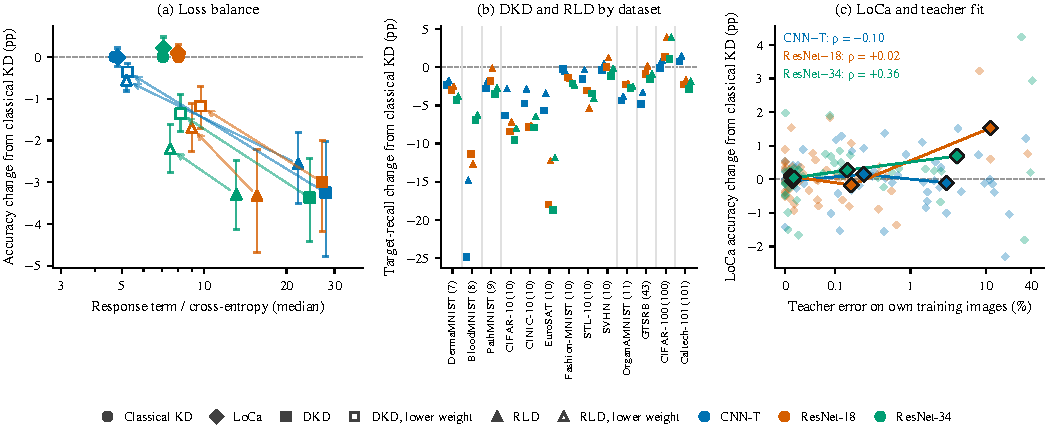
\includegraphics[width=\textwidth]{figures/loss_diagnostics.pdf}
\vspace{-4pt}
\caption{Diagnostics of the alternative losses with CNN-S as the
student. (a) Loss balance against the accuracy change from classical
KD, with arrows from each published loss to its lower-weight variant
and 95\% bootstrap intervals across settings. (b) Target-recall change
of the published DKD and RLD from classical KD on each dataset,
averaged over its four imbalance factors, with datasets ordered by class
count, given in parentheses. (c) LoCa's accuracy change from classical KD against the
teacher's error on its own augmented training images in the final
epoch, one point per setting, with Spearman's correlation $r_s$.}
\label{fig:loss-diagnostics}
\vspace{-6pt}
\end{figure*}

None of the three recent methods improved on classical KD in our
setting. LoCa matched it, staying within 0.4~pp in both metrics,
whereas DKD and RLD fell below it with every teacher
(Table~\ref{tab:loss-results}). We see three reasons, all tied to the
conditions of this study rather than to errors in the methods, and
Fig.~\ref{fig:loss-diagnostics} illustrates each. Color marks the
teacher and shape the loss. In (a), open markers are the lower-weight
variants, reached by arrows from the published weights; in (c), small
points are single settings and larger ones the mean change within
teacher training errors of up to 0.1\%, 0.1--1\% and above 1\%.

First, the published loss weights let the distillation term dominate
training. At those weights the median response term was 24 to 28 times
the cross-entropy for DKD and 13 to 22 times for RLD, against 5 to 8
times for classical KD (Fig.~\ref{fig:loss-diagnostics}a). A
distillation loss can limit how well the task loss
converges~\cite{zhao2023dot}, which fits the drop we observed. Lowering the response weight recovered 1.1 to
2.9~pp of accuracy, so the imbalance explains much of the gap. It does
not explain all of it, however, because the lower-weight variants still
trailed classical KD by 0.4 to 2.2~pp.

Second, both methods amplify the non-target part of the teacher's
prediction, and in our setting that part carries little and biased
information. DKD multiplies its non-target term by
$\lambda_{\mathrm{NC}}=8$ in Eq.~\eqref{eq:dkd-loss}~\cite{zhao2022decoupled}. RLD refines the teacher only where it
ranks another class above the ground truth~\cite{sun2025knowledge}, so
on correctly classified images its two terms reduce to target and
non-target matching in the same one-to-eight ratio. Ten of our 13
datasets have between seven and eleven classes, which leaves few
non-target probabilities to learn from. A teacher trained on
long-tailed data also shifts probability towards head
classes~\cite{huang2025learn}, and weighting those
probabilities eightfold pushes the student the same way, which is why
the published DKD lost more target recall than accuracy relative to
classical KD, 4.4 to 4.9~pp against 3.0 to 3.4~pp
(Table~\ref{tab:loss-results}). The shortfall varied widely across
datasets, however (Fig.~\ref{fig:loss-diagnostics}b). With every
teacher, the published DKD and RLD trailed classical KD in target
recall on at least nine of the ten datasets with seven to eleven
classes, by as much as 24.8~pp on BloodMNIST and 18.7~pp on EuroSAT,
whereas on CIFAR-100 they matched or exceeded it, by $-0.1$ to
$+3.9$~pp. Class count alone does not account for this. GTSRB and
Caltech-101, with 43 and 101 classes, still fell short in most cases,
and across the 13 datasets the rank correlation between class count
and the recall change was only 0.33 to 0.54 ($p\geq0.058$, Spearman).
The lower-weight variants followed the same pattern, though less clearly
with CNN-T. The shortfall was also larger with the ResNet teachers, where the
lower-weight variants trailed classical KD by 1.2 to 2.2~pp rather than
0.4 to 0.6~pp. A much larger teacher is also harder for a small
student to mimic~\cite{cho2019efficacy}.

Third, LoCa corrects the teacher only on training images that it
misclassifies~\cite{yang2024loca}, and our teachers rarely
misclassified them. In its final training epoch, the median teacher
classified 99.5\% of its own augmented training images correctly for
CNN-T and 99.9\% for both ResNets, so LoCa changed few targets and
stayed close to classical KD. Where a teacher fit its training images
less well, LoCa did gain more. The trend was clear with ResNet-34
($r_s=0.36$, $p=0.008$), appeared with ResNet-18 only in its three
settings above 1\% training error, and was absent with CNN-T
(Fig.~\ref{fig:loss-diagnostics}c). RLD also corrects only misclassified
images~\cite{sun2025knowledge}, yet it fell further behind classical KD
in accuracy where the teacher's training error was higher ($r_s$ from
$-0.32$ to $-0.56$), so this reason does not explain RLD's shortfall;
the first two do. A long-tailed teacher's bias
lies mainly in its confidence and in how it spreads probability across
classes, not in wrong top-1 predictions on the student's training
images, so a correction keyed to the label cannot reach it. Teacher repair instead edits the channels that produce those
probabilities, which may be why it improved the CNN-T students where
these losses did not.

These results agree with the observation that the advantage of refined
losses over vanilla KD depends on the data and the training
regime~\cite{hao2023revisit}. DKD and RLD were developed on CIFAR-100
and ImageNet, which have many classes, whereas our students are small,
most of our datasets have few classes and the training sets are
long-tailed. Here classical KD remains a strong
baseline, and further gains are more likely to come from improving what
the teacher provides than from changing how its output is matched.

\vspace{-5pt}
\subsection{From Localization to Transfer}
\label{sec:discussion-rqs}

We now return to the four research questions in
Section~\ref{subsec:approach}, and then to the choice between repairing
the teacher and changing the loss.

\textbf{RQ1.} The first question was whether a teacher's errors on the
target classes can be localized to a small set of parameters. In most
settings they can. Under the fixed budget, causal screening kept enough
channels to build a repair in 42 of the 52 settings for CNN-T, in every
setting for ResNet-18 and in all but one for ResNet-34
(Table~\ref{tab:teacher-architecture-results}). The selected repairs
edited two to eight channels, at most 4.2\% of CNN-T's searched
channels and about 1\% of a ResNet's, and editing only these channels
raised the teacher's target recall on the sealed test sets
(Section~\ref{sec:teacher-student-changes}). Localization did not
guarantee a repair, however. In many localized settings no candidate
improved validation target recall within the selection guardrail, so a
repair was selected in only 23, 18 and 21 settings.

\textbf{RQ2.} The second question was how editing the localized
parameters changes the teacher's decisions. The edits shifted specific
decisions rather than the model as a whole. Target recall rose roughly
three to five times as much as accuracy, by 2.68 against 0.87~pp for
CNN-T, 1.37 against 0.27~pp for ResNet-18 and 0.73 against 0.25~pp for
ResNet-34, so decisions moved towards the target classes while
accuracy still rose slightly. The edits also changed
the teacher's confidence, not only its top-1 predictions. For every
teacher, NLL, Brier score, ECE and AURC fell and selective accuracy rose
(Table~\ref{S-tab:secondary-results}), so the repaired teacher's
probabilities, which the student learns from,
became better calibrated and better separated right from wrong
predictions.

\textbf{RQ3.} The third question was whether that change survives
distillation. It survived in part, and most clearly with CNN-T. On
average, about half of the teacher's recall gain reached CNN-S: 58\%
with CNN-T, and 42\% and 56\% with ResNet-18 and ResNet-34. With CNN-T
this was enough to raise the student's accuracy and target recall
significantly over all 52 settings, and ten of the 23 repairs met the
transfer rule (Table~\ref{tab:overall-pair-results}). Its students were
also the most accurate and had the highest target recall of all the
methods we compared (Table~\ref{tab:loss-results}). With the ResNet
teachers the students' gains were small, reached significance only with
the scaled budget, and met the transfer rule in at most five repairs
per teacher. The students of every teacher also improved in all eight
additional metrics (Table~\ref{S-tab:secondary-results}), so the change
in the teacher's confidence carried over as well. Survival was not
guaranteed in any single setting, however. In one CIFAR-10 setting the
CNN-T teacher gained 5.14~pp of target recall, while its student lost
0.46~pp.

\textbf{RQ4.} The last question was what determines survival. The main
factor was the size of the teacher's gain. The share of that gain
reaching the student was similar for all three teachers, so the ResNet
students gained less chiefly because their teachers gained less. Across
settings, a larger teacher gain also indicated a larger student gain
for CNN-T and ResNet-18, though with substantial variation, but not for
ResNet-34, and the teacher's accuracy change indicated little for any
teacher (Section~\ref{sec:teacher-student-changes}). The channel budget
was not the limit. Scaling the ResNet budget fourfold changed neither
the teachers' nor the students' gains significantly
(Section~\ref{sec:teacher-architecture}). The size of the teacher's
gain was instead set by the teacher itself: repair raised CNN-T's target
recall about two and nearly four times as much as that of ResNet-18 and
ResNet-34. CNN-T is also much closer to the student in size, with 3.9
times its parameters against 149 and 284 times for the ResNets. Because
architecture and capacity gap change together in our design, separating
their effects will require larger students.

\textbf{Teacher or loss?} Our approach intervenes on the teacher rather
than on the loss (Section~\ref{subsec:approach}), and the comparison
with the alternative losses tests that choice directly. Changing the
loss did not help. LoCa matched classical KD, whereas DKD and RLD fell
below it with every teacher (Section~\ref{sec:discussion-losses}).
Changing the teacher did help, most clearly with CNN-T, where the
repaired-teacher student was the most accurate and had the highest
target recall of any method. With the ResNet teachers it was level with
classical KD and LoCa (Table~\ref{tab:loss-results}). Repairing the
teacher was therefore at least as effective as changing the loss, and
more effective with CNN-T. We ran the alternative losses only with the
original teacher, however, so our results cannot show whether combining
one with a repaired teacher would pass more of the repair to the
student, and we leave that combination to future work.

\FloatBarrier
\vspace{-5pt}
\section{Conclusion}
\label{sec:conclusion}

We asked whether repairing a teacher's errors on a designated set of
classes before distillation helps the student. Our repair edits only
the channels that causal screening links to those errors, at most
4.2\% of those it searches, and leaves classical KD unchanged. With
CNN-T as the teacher, it raised CNN-S's accuracy and target recall
significantly across 52 settings on 13 datasets and gave a better
student than LoCa, DKD and RLD. With the much larger ResNet teachers
the gains were small, even with a fourfold channel budget. Under the
fixed budget, about half of each teacher's recall gain reached the
student, so the student's gain depends mainly on how much repair
improves the teacher. Repairing the teacher therefore complements
refining the loss.

\textbf{Limitations.} CNN-S was the only student, so teacher
architecture and capacity gap changed together. All models used
$32\times32$ images, most datasets have few classes, and each setting
had a single trained teacher. Repair also kept the original teacher in
more than half of the settings, and we ran the alternative losses only
with the original teacher.

\textbf{Future work.} Students of several sizes would separate
architecture from the capacity gap. Because the ResNet repairs often
failed validation selection rather than localization, richer candidate
edits may help large teachers. Combining repair with a refined loss,
and testing both on larger benchmarks and transformer models, would
show how far the approach extends.

\FloatBarrier

% IEEE order: acknowledgments, then references.
% Uncomment and edit if required by the submission venue.
% \section*{Acknowledgments}
% The authors thank [name or funding source].

% Add and edit references in ref.bib, then cite them with \cite{citationKey}.
\bibliographystyle{IEEEtran}
\bibliography{ref}

\end{document}
